% Compile with: lualatex knights_tour.tex
\documentclass[11pt]{article}

\usepackage{amsmath, amssymb}
\usepackage{tikz}
\usepackage[a4paper, margin=2.5cm]{geometry}
\usepackage[colorlinks=true, urlcolor=blue]{hyperref}
\usepackage{fancyhdr}

\pagestyle{fancy}
\fancyhf{}
\renewcommand{\headrulewidth}{0pt}
\fancyfoot[L]{\small Junzhe Wang ~\textperiodcentered~
  \href{mailto:junzhe.wang2002@gmail.com}{\texttt{junzhe.wang2002@gmail.com}}}
\fancyfoot[R]{\small Last edited: \today\ ~\textperiodcentered~ p.\,\thepage}

\title{The Knight's Tour}
\author{}
\date{}

\begin{document}

\maketitle
\thispagestyle{fancy}

\section{The knight and its graph}

A knight on square $(x, y)$ may jump to any of the eight squares
\begin{equation}
  (x \pm 1, y \pm 2), \qquad (x \pm 2, y \pm 1)
\end{equation}
that lie on the board. Abstracting the chessboard away, the $N \times N$
\emph{knight graph} has one vertex per square and one edge per legal jump;
everything below is graph theory in chess clothing.

\begin{center}
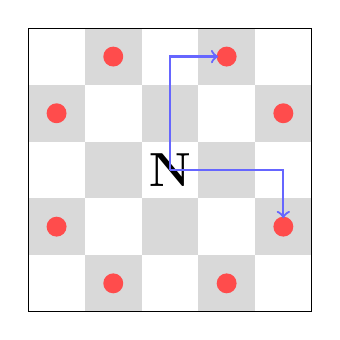
\begin{tikzpicture}[scale=0.72]
  \foreach \x in {0,...,4}
    \foreach \y in {0,...,4} {
      \pgfmathparse{mod(\x+\y,2) == 0 ? "white" : "black!15"}
      \edef\c{\pgfmathresult}
      \fill[\c] (\x, \y) rectangle ++(1, 1);
    }
  \draw (0, 0) rectangle (5, 5);
  \node at (2.5, 2.5) {\LARGE\bfseries N};
  \foreach \dx/\dy in {1/2, 2/1, 2/-1, 1/-2, -1/-2, -2/-1, -2/1, -1/2}
    \fill[red!70] (2.5 + \dx, 2.5 + \dy) circle (5pt);
  \draw[->, thick, blue!60] (2.5, 2.5) -- (2.5, 4.5) -- (3.35, 4.5);
  \draw[->, thick, blue!60] (2.5, 2.5) -- (4.5, 2.5) -- (4.5, 1.65);
\end{tikzpicture}

\smallskip
The eight knight moves; two are drawn as their L shapes.
\end{center}

\section{Open and closed tours}

A \emph{tour} visits every square of the board exactly once.
\begin{itemize}
  \item An \textbf{open tour} may end anywhere: a \emph{Hamiltonian path} of
    the knight graph.
  \item A \textbf{closed tour} (or re-entrant tour) ends a single knight's
    move away from its starting square, so the knight could go round
    forever: a \emph{Hamiltonian cycle}.
\end{itemize}

Existence is completely settled on square boards:
\begin{itemize}
  \item Open tours exist exactly for $N = 1$ and $N \geq 5$. There is no
    tour on $2 \times 2$ or $3 \times 3$ (on the latter, the center square
    has no knight move at all), and --- less obviously --- none on
    $4 \times 4$ either.
  \item Closed tours exist exactly for even $N \geq 6$.
\end{itemize}

The parity half of the closed-tour statement has a one-line proof worth
savoring. Every knight move changes square color, so any walk alternates
black and white. A closed tour is a cycle through all $N^2$ squares using
each exactly once; alternation around a cycle forces equally many squares
of each color, hence $N^2$ even, hence $N$ even. For odd $N$ the board has
one color in excess and no closed tour can exist --- an impossibility
established without examining a single candidate tour, just from an
invariant every move preserves.

\section{Algorithms}

\subsection{Backtracking}

The direct search extends a partial path square by square: from the current
square, try each unvisited neighbor in turn, recurse, and undo on failure;
success is a path of length $N^2$. This always works in principle --- it is
exhaustive --- but the knight graph is generous (up to eight choices per
step, path length $N^2$), and from an unlucky starting square the search
can wander through astronomically many dead ends before its first success.
Unlike the queens problem, where each placement prunes entire columns and
diagonals, a knight move constrains the future only weakly.

\subsection{Warnsdorff's rule}

The classical remedy (1823) is a greedy ordering: \emph{always jump to the
unvisited square that itself has the fewest unvisited onward moves}. The
intuition is a scheduling principle: squares with few remaining accesses
are the ones in danger of becoming unreachable, so they must be consumed
first; well-connected squares can wait. With this ordering the very first
descent of the search almost always completes the tour --- backtracking in
name, linear in practice.

Two honest caveats. Ties (several squares with the same minimal degree)
must be broken somehow, and on larger boards a poor tie-breaking rule can
strand the pure heuristic in a dead end; keeping the backtracking machinery
underneath restores certainty at no cost when the heuristic behaves. And
greedy success is empirical, not guaranteed: the rule is a heuristic, not a
theorem.

\section{From mathematics to program}

The program searches for \emph{closed} tours. It represents the board as a
visited matrix plus the trail of moves so far; the eight jump offsets are a
constant list. A candidate is accepted when the path covers all $N^2$
squares \emph{and} its last square is a knight's move from the first ---
the extra closure test is the only difference from an open-tour search.
The result is an \emph{option}: \texttt{Some tour} on first success ---
there is no point enumerating further --- or \texttt{None}, which for odd
$N$ or $N < 6$ is not a failure of the search but a fact of mathematics.
Sorting candidate moves by onward degree turns the naive search into
Warnsdorff's; timing both against each other makes the difference
measurable rather than anecdotal.

\end{document}
